\documentclass[
course = {{Mecánica Cuántica II}}
]{aga-homework}
\usepackage{physics}
\newcommand{\up}[1]{^{#1}}
\begin{document}

\title{\vspace{-30pt}Trabajo: Mecánica Cuántica II}

\author{Andrea Verona Velásquez,\\
Jesús Manuel Gallego Mercado,\\
Luis Miguel Patiño Buendía}

\maketitle

\section*{Ejercicios, María Carolina Espinel}
\subsection*{Ejercicio 2, Pág 405:} Considere el sistema del oscilador armónico isotrópico. Determine la ecuación de valores propios en representación de coordenadas empleando coordenadas esféricas. Muestre que en la ecuación de Schrödinger independiente del tiempo la variable radial se puede separar de las variables angulares. Encuentre la ecuación diferencial para la parte radial de la función de onda y averigüe cuáles son sus soluciones. Compare sus resultados con los obtenidos en el capítulo 3.

\subsection*{Ejercicio 3, Pág 420}
Demuestre que el degeneramiento de los valores propios de energía de un átomo hidrogenoide sin espín es $n^2$. Tengo en cuenta que $\sum_{k=1}^{N} k = N(N+1)/2$.

\subsection*{Ejercicio 4, Pág 420}
Supongo que en $t=0$ el estado del electrón de un átomo de hidrógeno (sin espín) está dado por $\psi(\vb{r}, 0)=1/\sqrt{5}\qty{\varphi_{3,1,1}(\vb{r})+2\varphi_{3,2,1}(\vb{r})}$, donde $\qty{\varphi_{n,l,m_{l}}}$ es el conjunto de funciones propias del hamiltoniano electrónico. ¿De cuál (o cuáles) operadores del conjunto $\qty{\vu{H},\vu{L}^2, \vu{L}_z}$ es ket propio este estado inicial? Calcule el valor esperado, o promedio, de los operadores del conjunto para $t>0$. ¿Se conservan los valores esperados? ¿Esperaba estas respuestas? Justifique.

\subsection*{Ejercicio 5, Pág 421}
Suponga que en $t=0$ el estado del electrón de un átomo de hidrógeno (sin espín) está dado por $\ket{\psi(0)}=1/\sqrt{5}\qty{\ket{1,0,0} + 2\ket{2,0,0}}$ calcule para $t>0$ el valor esperado del operador $\vu{r}$ ¿Cambia en el tiempo el valor esperado? ¿Esperaba esta respuesta? Justifique.

\section*{Segunda parte del Trabajo}
\subsection*{Ejercicio 1.}
Revisar el libro de Constantinescu en la pag. 77 problemas números 6 y 7 sobre la deducción de la fórmula de Kramers y luego revisar las paginas 81 en adelante para ver la solución de los mismos estos deben revisarse y complementar los pasos intermedios faltantes en la demostración. Finalmente aplique lo anterior para obtener la expresión 6.3.20 de la Página 416/456 del libro de Maria Carolina Spinel.

\subsection*{Ejercicio 2.}
Del libro de Constantinescu en la página 31(37 del documento) los  números 30,  31 y 33. Revisar las soluciones que se encuentran en el mismo libro y complementar los pasos intermedios faltantes.\\

\textbf{Solución:} 

\subsubsection*{Ejercicio 30.}
Encuentre las posibles energías de una partícula en el potencial esférico dado por $V(r) = -V_0$ si $r<a$ y $V(r)=0$ si $r>a$. (revise Fig \ref{fig:luis_img0}).

\begin{figure}
    \centering
    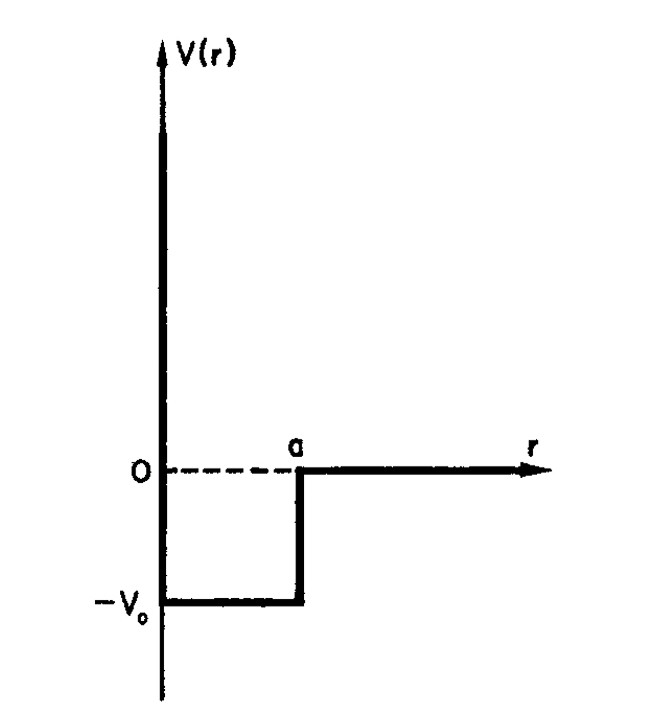
\includegraphics[width=0.3\columnwidth]{img/luis_img0}
    \caption{Potencial $V(r)$}
    \label{fig:luis_img0}
\end{figure}

\subsubsection*{Ejercicio 31.}
Encuentre los niveles de energía de una partícula en un campo central:

\begin{gather}
V(r) = \frac{A}{r\up{2}}+B r\up{2},
\end{gather}

donde $A$ y $B$ son constantes positivas.
Demostrar que, en el caso particular $A=0$, $B=\frac{1}{2}m\omega\up{2}$, los niveles son los mismos que los encontrados en el problema 20 para un oscilador isotrópico tridimensional.
\end{document}
